% Chapter 4 documents data evidence and representation choices for newline-only alignment.
% Focus: dataset scope, dataset-specific composition, shared artifacts, preprocessing, and data-level validity limits.

\chapter{Data}
\label{cha:data}

\section{Dataset Portfolio and Evaluation Scope}
\label{sec:data_portfolio}
\label{sec:data_scope_role}

Newline-only alignment is evaluated at the intersection of two kinds of evidence: A fixed transcription character sequence and the line structure visible or annotated in document images. A useful test portfolio therefore needs more than transcriptions alone. It must expose how page images, line-broken ground truth, optical character recognition/handwritten text recognition (OCR/HTR) hints, and line-level image evidence can be connected to the same sample without pretending that all datasets provide those artifacts in the same way \thesiscite{fischer2011icdarInaccurateAlignment,hassner2013ocrFreeAlignment}.

The empirical evidence base is specified for the task defined in \autoref{sec:theory_problem_definition}. The account is intentionally descriptive: It reports data composition, provenance, artifact availability, preprocessing, and quality considerations, but does not report method performance. This separation follows standard evaluation practice in document analysis, where protocol and data specification are fixed before method comparison \thesiscite{clausner2011scenarioDrivenEval,vidal2023pageLevelAssessment}.

The evaluation portfolio is handwritten-first. The main evidence layer consists of four handwritten datasets: Bullinger Handwritten, Children Handwritten, IAM Handwritten, and Washington Handwritten. Together they cover historical correspondence, modern benchmark handwriting, restricted AIBEX-provided child handwriting, and eighteenth-century manuscript pages. The printed versions of Bullinger and IAM are used as supporting printed context for the same newline-only task. The printed context was evaluated only for the raw-output configurations because of computational and API budget constraints, and evaluation resources were prioritized for handwriting because handwritten line boundaries are generally harder to recover and many target historical-document collections are handwritten. The printed rows therefore broaden the modality picture without changing the handwritten-first scope of the thesis.

Table~\ref{tab:data_dataset_inventory} gives the dataset inventory used by this chapter. In each row, \(n\) denotes the number of evaluated samples: Handwritten or printed letter samples for Bullinger, page-image samples for Children and Washington, forms for IAM Handwritten, and form/page entries for IAM Print. Lines are stored ground-truth lines. Character counts are Unicode code points after removing newline separators, so they measure transcription volume rather than layout markup. The table is an inventory and role table only; it does not report accuracy.

\begin{table}[H]
  \centering
  \caption{Dataset inventory and evaluation role. The handwritten rows form the primary evaluation portfolio. The printed rows provide additional modality context. The \(n\) column reports the number of evaluated samples for each row.}
  \label{tab:data_dataset_inventory}
  \footnotesize
  \renewcommand{\arraystretch}{1.08}
  \setlength{\tabcolsep}{3.2pt}
  \begin{tabularx}{\linewidth}{@{}>{\raggedright\arraybackslash}p{0.20\linewidth}>{\raggedright\arraybackslash}p{0.13\linewidth}>{\raggedleft\arraybackslash}p{0.055\linewidth}>{\raggedleft\arraybackslash}p{0.06\linewidth}>{\raggedleft\arraybackslash}p{0.07\linewidth}>{\raggedleft\arraybackslash}p{0.08\linewidth}>{\raggedright\arraybackslash}X@{}}
    \toprule
    \textbf{Dataset} & \textbf{Modality} & \textbf{\(n\)} & \textbf{Pages} & \textbf{Lines} & \textbf{Chars} & \textbf{Evaluation role} \\
    \midrule
    Bullinger Handwritten & handwritten & 59 & 100 & 2{,}535 & 133{,}883 & primary handwritten evaluation \\
    Bullinger Print & printed & 10 & 10 & 271 & 15{,}004 & additional printed context \\
    Children Handwritten & handwritten & 63 & 63 & 394 & 10{,}261 & primary handwritten evaluation \\
    IAM Handwritten & handwritten & 20 & 20 & 180 & 7{,}604 & primary handwritten evaluation on representative-20 subset \\
    IAM Print & printed & 30 & 30 & 161 & 12{,}194 & additional printed context \\
    Washington Handwritten & handwritten & 20 & 20 & 656 & 26{,}458 & primary handwritten evaluation \\
    \bottomrule
  \end{tabularx}
\end{table}

\section{Datasets}
\label{sec:data_datasets}

The dataset-level discussion below follows this handwritten-first structure. Bullinger Handwritten and Washington Handwritten represent historical manuscript material, where page condition, historical spelling, and irregular layout make line placement a central part of transcription interpretation \thesiscite{peer2025ctcBullingerAlignment,lavrenko2004holisticWordRecognition}. IAM Handwritten is the public benchmark anchor for modern English handwriting, while Children Handwritten adds restricted AIBEX-provided child handwriting with different writer and language characteristics \thesiscite{marti2002iam}. The printed versions of Bullinger and IAM add printed layouts so the same newline-only target can be inspected outside handwriting, while remaining supporting context rather than a parallel full evaluation track.

Using selected examples from the four evaluated handwritten datasets, Figure~\ref{fig:data_handwritten_page_examples} uses enlarged line-region crops to make the visual heterogeneity of the handwritten portfolio explicit without repeating the task illustration from \autoref{fig:intro_newline_alignment_task}. The comparison foregrounds differences in line density, baseline regularity, ruling, and document condition that directly affect how confidently newline positions can be recovered from page-side or line-level evidence.

\begin{figure}[H]
  \centering
  \subfigure[Bullinger.]{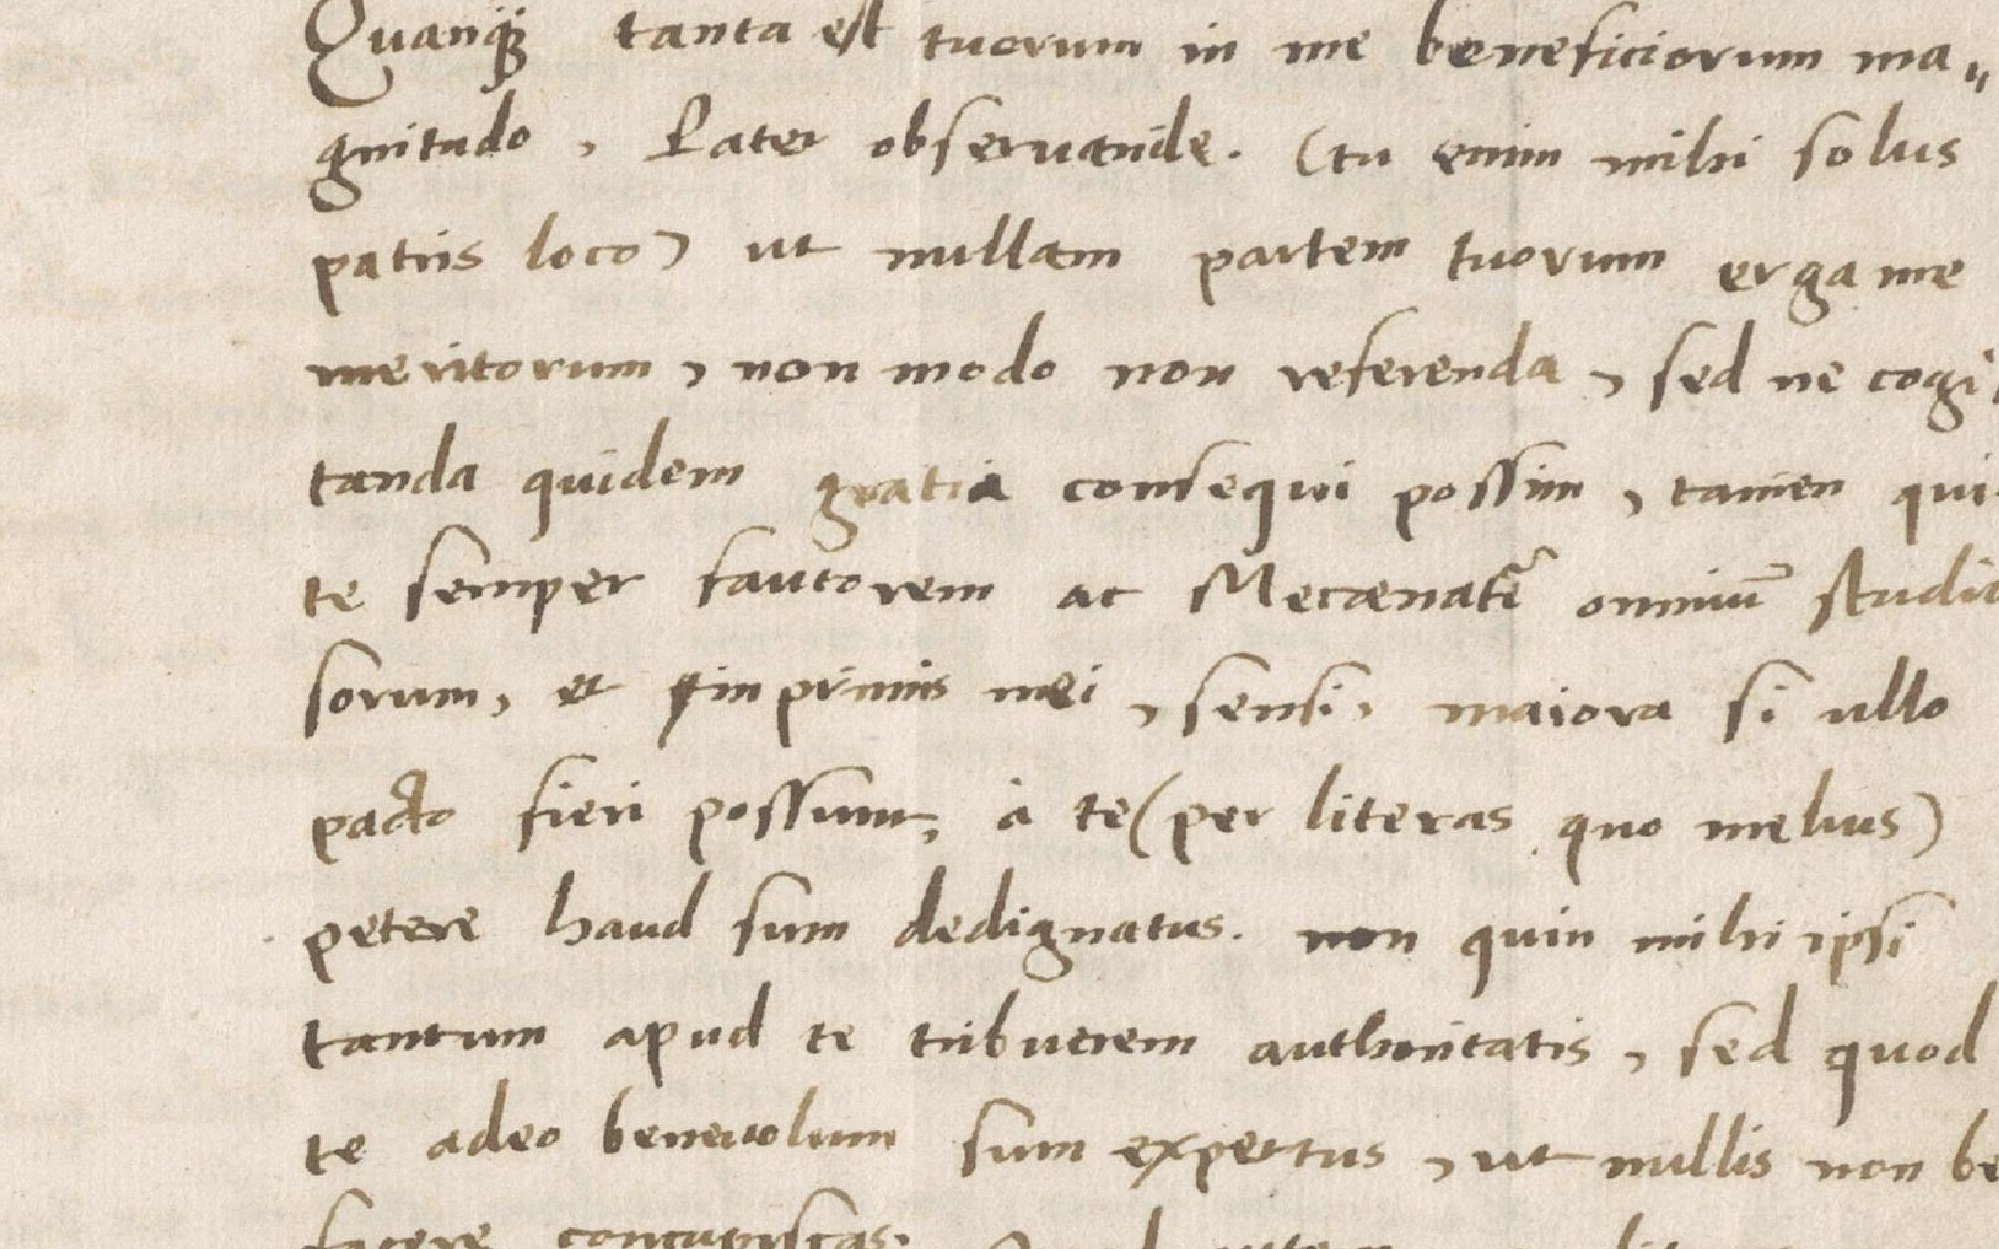
\includegraphics[width=0.47\textwidth]{images/pdf_optimized/ch4_bullinger_10333_0001_crop.jpg}}
  \hfill
  \subfigure[Children.]{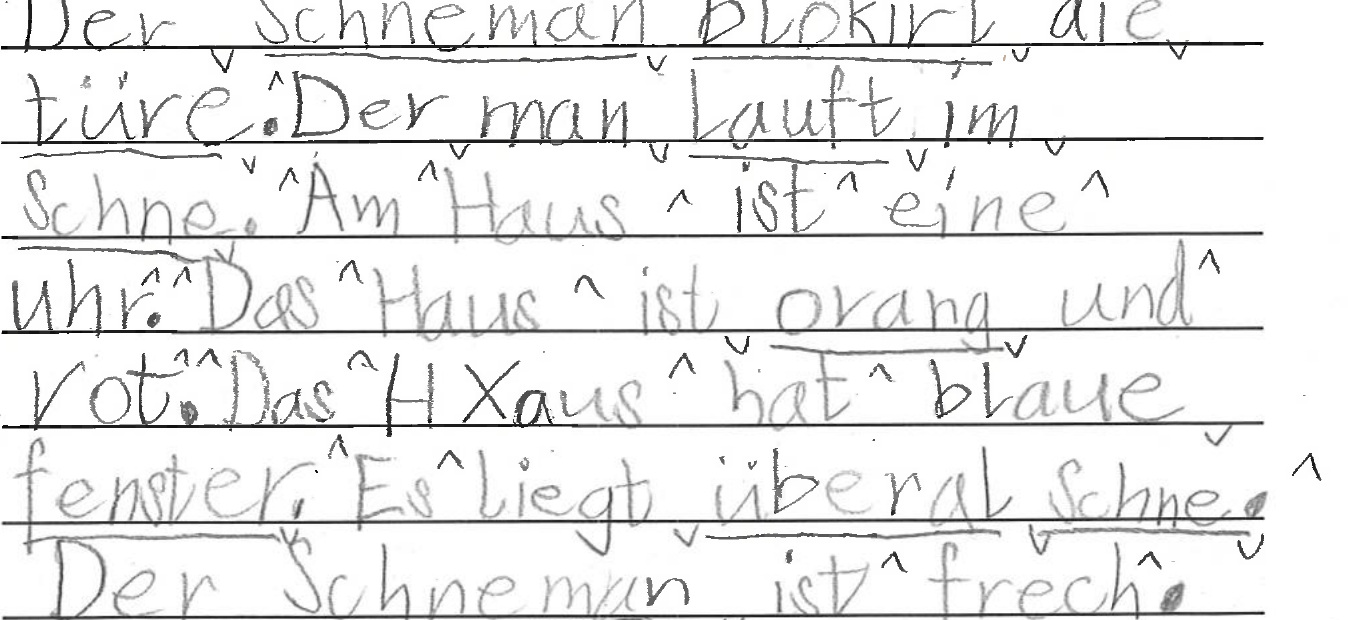
\includegraphics[width=0.47\textwidth]{images/pdf_optimized/ch4_children_1A_17_2_crop.jpg}}

  \vspace{0.6em}

  \subfigure[IAM.]{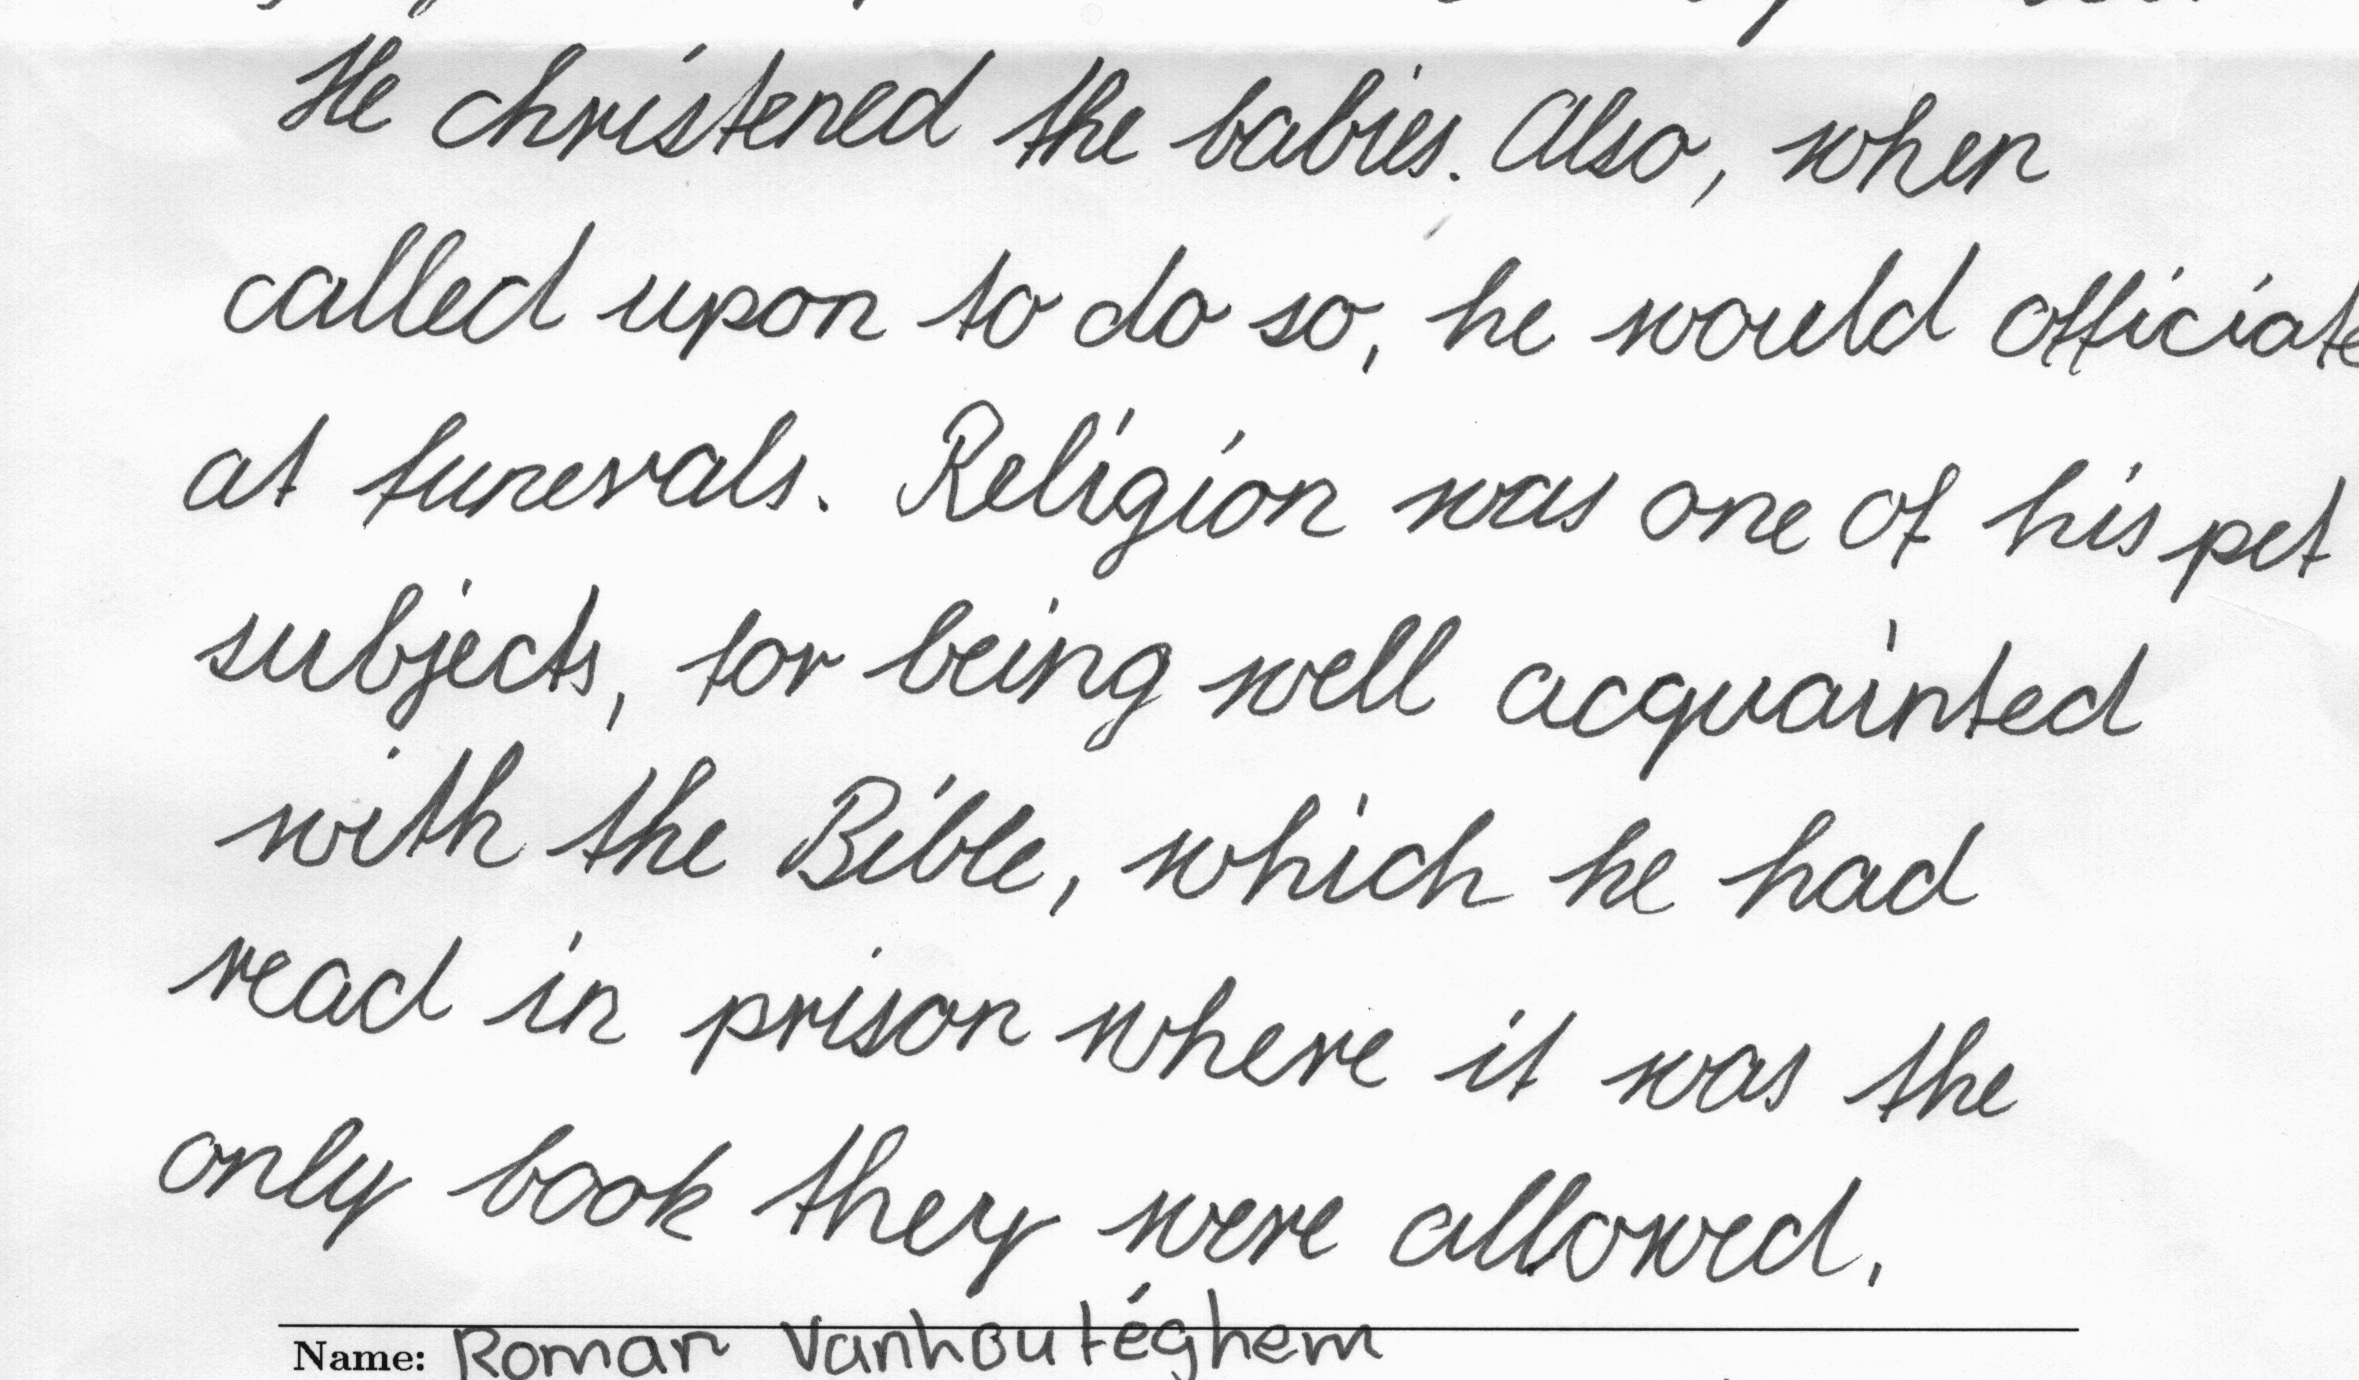
\includegraphics[width=0.47\textwidth]{images/pdf_optimized/ch4_iam_rep20_g03-043_crop.jpg}}
  \hfill
  \subfigure[Washington.]{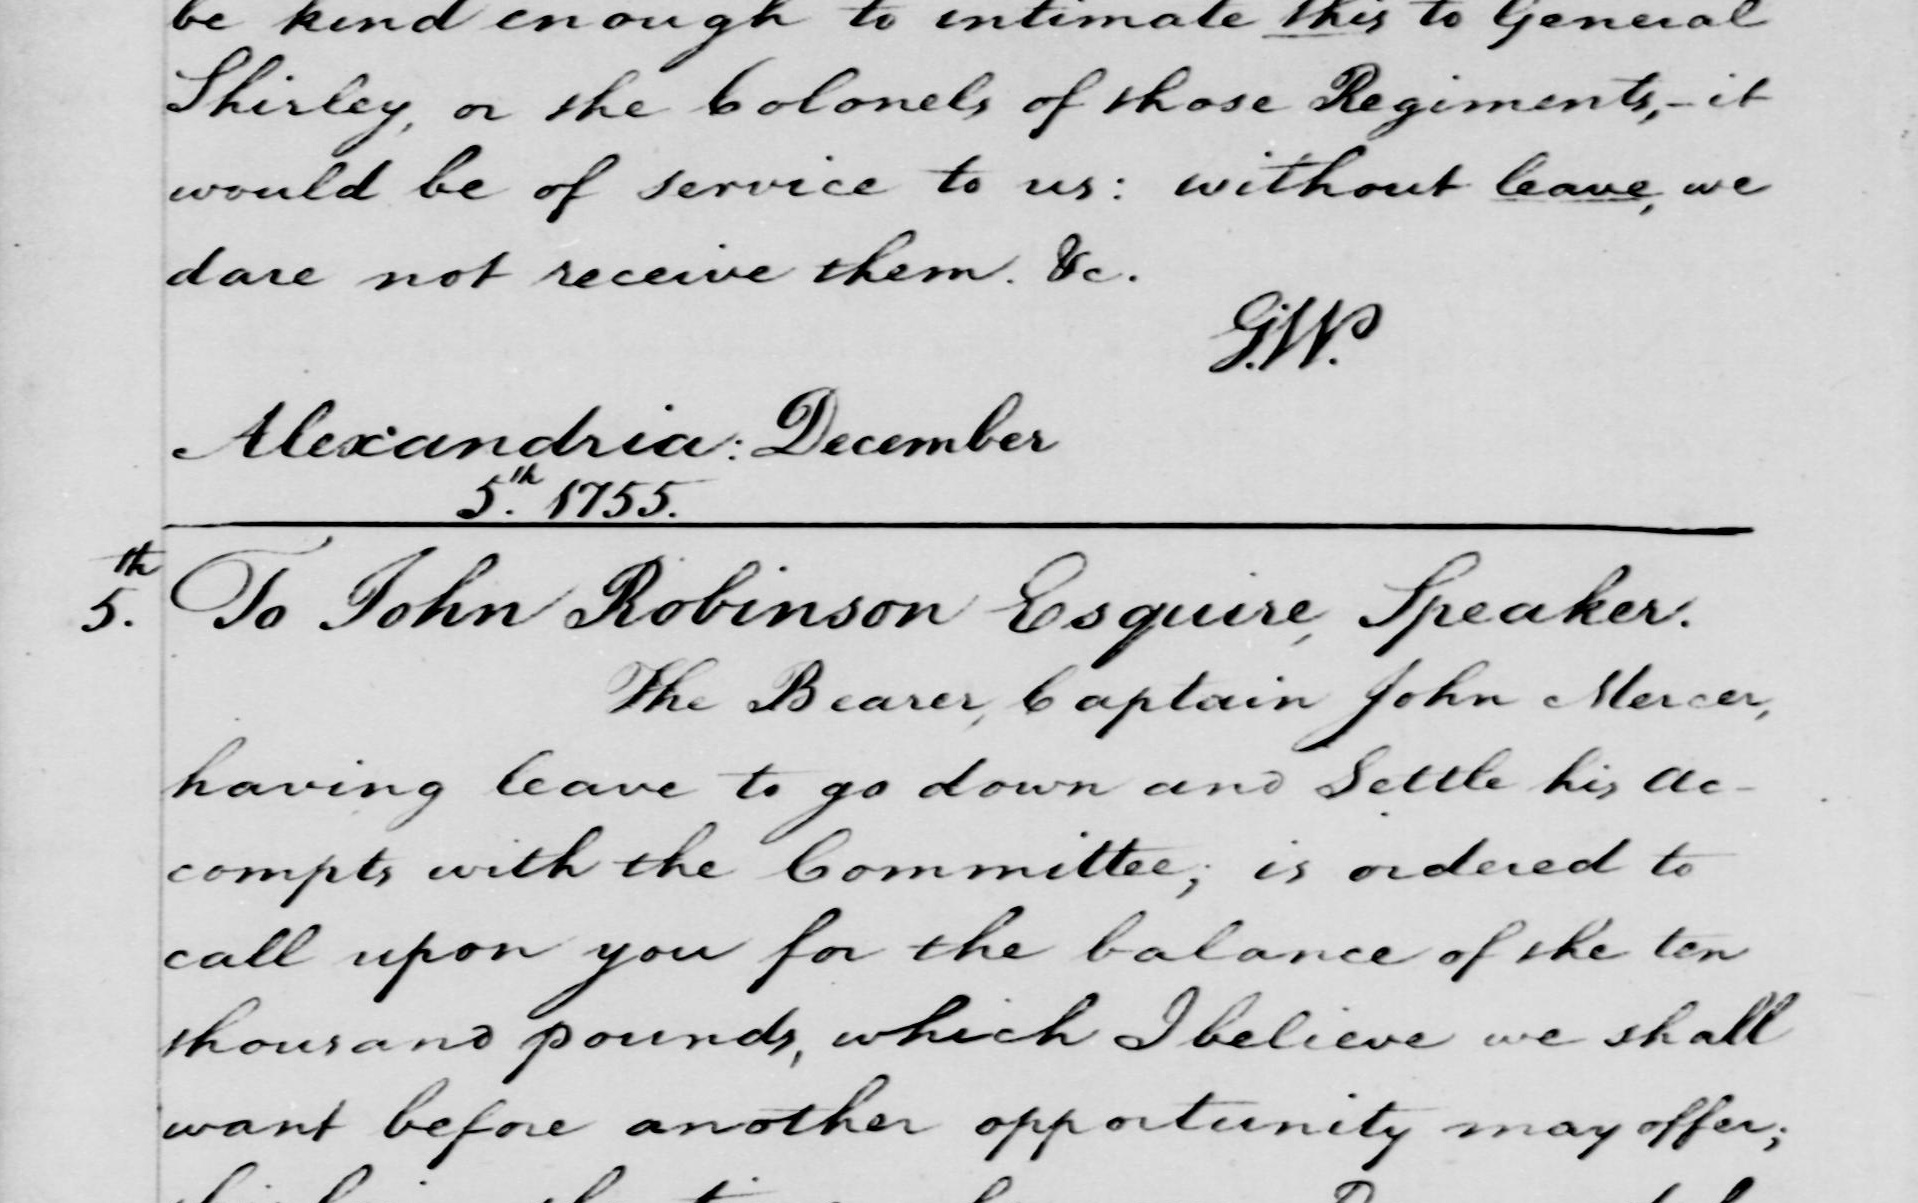
\includegraphics[width=0.47\textwidth]{images/pdf_optimized/ch4_washington_304_crop.jpg}}
  \caption{Cropped line-region examples from the four handwritten evaluation datasets. The panels emphasize visual heterogeneity across dense historical writing, ruled child handwriting, regular IAM forms, and degraded or structured Washington pages.}
  \label{fig:data_handwritten_page_examples}
\end{figure}

\subsection{Bullinger Handwritten and Print}
\label{sec:data_bullinger}

Bullinger Handwritten is a historical correspondence subset consisting of 59 letter-level samples. The reported count therefore refers to letter/sample IDs rather than single pages: Together, the samples span 100 page images and 2{,}535 ground-truth lines. For this thesis, the evaluation set combines two author-provided parts: Subset~1 contributes 20 letters, 50 pages, and 902 lines, while Subset~2 contributes 39 letters, 50 pages, and 1{,}633 lines. This composition matters because Bullinger contributes dense correspondence layouts, multilingual and premodern writing practices, and manuscript-specific line-boundary ambiguity \thesiscite{peer2025ctcBullingerAlignment,nikolaidou2022historicalDatasetSurvey}.

The broader Bullinger dataset is linguistically diverse, primarily Latin and premodern German, with passages in Greek, Italian, French, and Hebrew \thesiscite{peer2025ctcBullingerAlignment}. In the evaluation staging, PAGE/XML annotations provide the line order and line crops, and the stored structured line metadata matches the ground-truth line count on all 59 handwritten samples. This means that the staged data contains PAGE/XML-derived line order and known line counts; it is not evidence for blind page-side line detection.

\paragraph{Bullinger version note.}
The Bullinger subset used in this thesis is an author-provided version shared by Marco Peer. A provenance note from the author correspondence records that this subset version is acceptable for thesis use and that reevaluating all Bullinger runs consistently on that same subset keeps the thesis-side comparisons fair.\footnote{Provenance information, not a bibliographic source: Marco Peer, email communication with the author, 22 April 2026. The note also records that the final paper subset was not published in exactly the same form, that letter swaps after contamination checks introduced version drift relative to the paper description, and that the final official Subset~2 inventory may contain 1483 rather than 1486 lines.} Chapter~\ref{cha:experimentation} therefore separates the fairness of the internal thesis comparisons from the specific question of direct comparability in the Bullinger published-baseline comparison. The published Bullinger study remains cited as the external source for the dataset and reported baseline context \thesiscite{peer2025ctcBullingerAlignment}.

Bullinger Print is the printed Bullinger counterpart used as supporting context. It contains 10 printed Bullinger letter samples, each represented by one page image, for a total of 271 ground-truth lines. It preserves part of the historical-document setting while replacing handwriting with printed typography, making it useful for inspecting how the newline-only task behaves under a different visual modality. In the evaluation staging for this thesis, it provides page images, fixed transcriptions, line-broken ground truth, and OCR text; structured line metadata and line-image crops are not part of this printed staging.

For Bullinger, the retained printed-context artifacts also include a same-ID handwritten support slice for M1--M3. This makes a restricted print--handwriting comparison possible on the shared support IDs, but it does not change the main 59-sample Bullinger Handwritten denominator used for the primary handwritten evaluation.

\subsection{Children Handwritten}
\label{sec:data_children}

Children Handwritten contains unpublished AIBEX-provided handwritten material. The reported count means 63 evaluated handwritten samples, each represented by one page image, for a total of 394 ground-truth lines. It adds modern child handwriting to a portfolio otherwise dominated by historical manuscript and public benchmark material. The relevant variation is writer age, school-writing context, German language material, and child-specific spelling and orthographic variation.

The evaluation staging preserves dataset-provided presegmented line-image folders from the controlled source export and standardizes their order. The resulting line-image inventory contains one line crop per ground-truth line, and the stored structured line metadata matches the ground-truth line count on all 63 samples. No public per-sample language metadata is available for this restricted export, so the chapter describes language and provenance only at aggregate level.

\paragraph{Children Handwritten governance note.}
Children Handwritten is restricted AIBEX-provided evaluation material. The thesis reports aggregate evaluation results and includes only supervisor- or dataset-owner-approved short qualitative excerpts and selected illustrative cropped images needed for analysis. The underlying dataset, full page images, full per-sample transcriptions, source manifests, and controlled export files are not redistributed with this thesis. Any external reuse or redistribution requires approval from the dataset owner or supervisor.

Children Handwritten remains reproducible only for researchers who have access to the controlled AIBEX source export. The thesis can disclose the dataset-level denominators, build logic, and evaluation code, but not the underlying images, per-sample transcriptions, or the controlled source manifest. External reruns therefore require the same restricted source export and owner approval; without that access, the thesis supports protocol transparency but not fully public package-level replication.

\subsection{IAM Handwritten and Print}
\label{sec:data_iam}

IAM Handwritten denotes the fixed 20-form representative subset used in the thesis, not the full IAM handwriting collection. The reported count therefore means 20 IAM forms, each treated as one page/form sample, for a total of 180 ground-truth lines. The subset is materialized as an explicit form list rather than generated by random sampling at evaluation time. Within that fixed subset, the 20 forms span 17 writer prefixes and cover a 4--12 lines-per-form range, compared with 4--13 in the full RWTH test split. The IAM database and the RWTH split provide the public benchmark anchor for modern English handwriting \thesiscite{marti2002iam,zimmermann2002iamSeg,openslr56iam}.

IAM Handwritten contributes controlled modern handwriting with public provenance and official IAM form and line images. The thesis staging uses the official IAM line indices within each form; the stored structured line metadata over official IAM line images matches the ground-truth line count on all 20 forms. This makes IAM useful as a comparatively regular, public, modern handwriting anchor rather than as another historical collection.

IAM Print contains the machine-printed IAM text regions staged as printed form/page samples. The reported count means 30 forms/pages in the staged dataset, totaling 161 ground-truth print lines. It is printed, not handwritten, and it is not the same denominator as the 20-form handwritten representative subset. As supporting printed context, it adds a clean, modern counterpart to the handwritten IAM material while preserving the same general form/page source family. Its modality contribution lies in regular typography and short printed line blocks. Like Bullinger Print, it provides page images, fixed transcriptions, line-broken ground truth, and OCR text; structured line metadata and line-image crops are not part of this printed staging.

For IAM, the retained printed-context artifacts include a paired 30-form \texttt{a01-*} handwritten support slice for M1--M3. This paired slice supports a direct diagnostic print--handwriting comparison in Chapter~\ref{cha:experimentation}, but it is separate from the fixed representative-20 IAM Handwritten denominator used in the main evaluation.

\subsection{Washington Handwritten}
\label{sec:data_washington}

Washington Handwritten contains a 20-page historical handwritten evaluation set. The reported count means 20 page samples, each represented by one page image, for a total of 656 ground-truth lines. It contributes eighteenth-century English manuscript writing with a different historical source, page style, and degradation profile from Bullinger \thesiscite{lavrenko2004holisticWordRecognition}. In the portfolio, Washington therefore adds historical English writing, relatively dense page-level line structure, and a separate manuscript tradition.

Washington Handwritten uses a reviewed crop layer derived from a raw Kraken segmentation workspace. The evaluation version preserves the raw segmentation manifests separately and then rewrites the final staged crop inventory through reviewed merge, drop, split, insert, and bounding-box edits until the staged crop count matches the ground-truth line count on every evaluated page. The data boundary is therefore explicit: The staged version contains a curated one-crop-per-line inventory for alignment, not a blind page-side line-detection benchmark.

\section{Shared Artifacts and Preprocessing}
\label{sec:data_representation}
\label{sec:data_handwritten_artifact_availability}
\label{sec:data_ocr_provenance}

The six staged datasets share the same core sample schema: Line-broken ground truth, fixed transcription without line breaks, page images, and OCR/HTR text. The primary handwritten datasets additionally have structured line metadata in \texttt{ocr\_lines} records and line-image crops for every evaluated sample. The printed-context datasets do not include structured line metadata or line-image crop inventories in the staged datasets.

All evaluation datasets follow a common artifact representation per sample ID:
\begin{itemize}
  \item Ground truth text with line breaks,
  \item Fixed transcription without line breaks,
  \item Page image sequence,
  \item \OCRHTR text with line breaks,
  \item Ordered structured line metadata and line-image crops for the primary handwritten datasets.
\end{itemize}
This harmonization keeps the newline insertion target constant while allowing the later chapters to distinguish which evidence is available for each dataset. Table~\ref{tab:data_artifact_semantics} summarizes how each artifact maps to its task role.

Let sample $s$ be represented by
\[
(g_s, x_s, v_s, o_s, L_s),
\]
where $g_s$ denotes line-broken ground truth, $x_s$ the fixed transcription without line breaks, $v_s$ the ordered page-image sequence, $o_s$ the \OCRHTR output used as structural hint text, and $L_s$ the ordered line-image crop sequence when available or derivable. Relative to \autoref{sec:theory_problem_definition}, $x_s$ is the fixed character stream and only newline boundaries are predicted; $g_s$ is used exclusively for evaluation, while $o_s$ and $L_s$ serve as auxiliary structural evidence.

\begin{table}[H]
  \centering
  \caption{Artifact semantics per sample.}
  \label{tab:data_artifact_semantics}
  \begin{tabular}{@{}p{2.2cm}p{6.25cm}p{4.75cm}@{}}
    \toprule
    \textbf{Artifact} & \textbf{Semantics} & \textbf{Task role} \\
    \midrule
    $g_s$ & line-broken ground truth text for metric computation only & evaluation only \\
    $x_s$ & fixed transcription without line breaks & fixed character stream for newline insertion \\
    $v_s$ & ordered page images, single-page or multi-page depending on sample & page-level visual evidence \\
    $o_s$ & \OCRHTR text with line breaks as noisy structural hint & auxiliary textual line-structure evidence \\
    $L_s$ & ordered line-image crops from segmentation or dataset-provided line folders & line-level visual evidence where staged \\
    \bottomrule
  \end{tabular}
\end{table}

Table~\ref{tab:data_handwritten_artifact_availability} records the provenance of the handwritten line-level evidence. All four handwritten datasets provide complete sample-level coverage for page images, fixed transcriptions without line breaks, line-broken ground truth, \OCRHTR text, structured \texttt{ocr\_lines} JavaScript Object Notation (JSON), and line-image crops. The asymmetry is not whether line-level evidence exists, but how that evidence is produced and how line order and expected line count are fixed.

\begin{table}[H]
  \centering
  \caption{Line-level evidence provenance on the four handwritten evaluation datasets. Page images, fixed transcriptions, line-broken ground truth, \OCRHTR text, structured \OCRLinesPath{} metadata, and line-image crops are available for all evaluated handwritten samples; the table highlights the provenance dimensions that differ across datasets and constrain leakage, known-count assumptions, and reproducibility claims.}
  \label{tab:data_handwritten_artifact_availability}
  \footnotesize
  \renewcommand{\arraystretch}{1.08}
  \begin{tabularx}{\linewidth}{@{}>{\raggedright\arraybackslash}p{0.15\linewidth}>{\raggedright\arraybackslash}Y>{\raggedright\arraybackslash}Y>{\raggedright\arraybackslash}Y>{\raggedright\arraybackslash}Y@{}}
    \toprule
    \textbf{Dataset} & \textbf{Line-crop provenance} & \textbf{OCR-line text provenance} & \textbf{Source of line order} & \textbf{Expected line count source} \\
    \midrule
    Bullinger Handwritten (\(n=59\) letter samples) & PAGE/XML-derived line crops materialized from the author-provided Bullinger export & PyLaia OCR over PAGE/XML-derived line images & PAGE reading order from XML & stored \texttt{ocr\_lines} cardinality over PAGE/XML-derived lines; equals ground truth on 59/59 samples \\
    Children Handwritten (\(n=63\) samples) & dataset-provided presegmented line-image folders copied from the controlled source export & PyLaia OCR over dataset-provided line images & dataset crop order preserved by standardized line renaming in dataset build & stored \texttt{ocr\_lines} cardinality over dataset-provided line folders; equals ground truth on 63/63 samples \\
    IAM Handwritten (\(n=20\) forms) & official IAM line images staged from the RWTH test split & PyLaia OCR over official IAM line images & official IAM line indices within each form & stored \texttt{ocr\_lines} cardinality over official IAM line images; equals ground truth on 20/20 forms \\
    Washington Handwritten (\(n=20\) page samples) & curated Kraken crops from the reviewed Washington alignment workspace; staged inventory contains one crop per ground-truth line & OCR scaffold over the curated Kraken crop inventory & curated review order materialized into final \texttt{line\_index} order & stored \texttt{ocr\_lines} cardinality over curated one-crop-per-line staging; equals ground truth on 20/20 samples \\
    \bottomrule
  \end{tabularx}
\end{table}

The OCR/HTR hint artifact $o_s$ is generated by a unified pipeline that first segments page images into line crops and then recognizes each crop as text. At software level, the implementation supports Kraken segmentation \thesiscite{kiessling2025kraken}, TrOCR recognition presets \thesiscite{li2023trocr}, optional docTR segmentation \thesiscite{mindee2026doctr}, and passthrough reuse of already segmented line folders. Dataset-specific choices are summarized in Table~\ref{tab:data_handwritten_artifact_availability}; the printed-context datasets use printed-recognition OCR hints but not the handwritten structured line-crop layer.

For multi-page samples, recognized text is concatenated in page order with explicit page-level separation, preserving sample-level sequence semantics for downstream alignment. Cacheable line crops and optional metadata sidecars are used to make \OCRHTR generation repeatable across reruns and cluster jobs; the reusable artifact chain is summarized in Table~\ref{tab:method_reproducibility_artifacts}.

\section{Data Quality and Validity Considerations}
\label{sec:data_threats}

Dataset heterogeneity is both a strength and a risk: Mixing historical and modern material improves coverage but increases variance in writing style, page condition, and language conventions. Domain shift under OCR noise is known to alter downstream textual behavior, so conclusions should be interpreted per dataset first and only then aggregated \thesiscite{nikolaidou2022historicalDatasetSurvey,marz2021dataCentricDomainAdaptation}.

At line level, annotation and boundary ambiguity remain inherent in historical documents because multiple nearby separators can be plausible under touching strokes, skew, bleed-through, or marginal additions. Therefore, absolute score differences should be interpreted together with qualitative evidence and complementary metrics rather than as purely geometric truth/falsehood decisions \thesiscite{likformansulem2006textLineSurvey,gruning2018readbad}.

A known-count assumption is a construct-validity boundary for the structured handwritten rows discussed in later chapters. The stored \texttt{ocr\_lines} payload provides the expected number of output lines, and that cardinality matches the ground-truth line count on every evaluated handwritten sample. This is especially important for Washington Handwritten, where the committed crop layer is curated until the staged inventory contains one crop per ground-truth line. These settings are still informative for newline placement under aligned line evidence, but they should not be interpreted as blind end-to-end page segmentation or page-side line-count prediction.

OCR/HTR enters the evaluation as auxiliary structural evidence rather than as the target to be scored. Whenever a regime relies on OCR/HTR text or structured OCR-line metadata, recognition errors can propagate into boundary suggestions. This creates a dependency between OCR quality and alignment outcomes that does not exist in purely image-guided settings, and it motivates keeping OCR-conditioned evidence analytically separate from image-side evidence in later reporting \thesiscite{li2023trocr,liu2024ocrbench}.

Where ordered line-image crops are used, line-level evidence quality becomes the critical dependency. Segmentation mistakes, crop ordering errors, or incomplete line folders can degrade alignment even when the downstream model or recognizer is otherwise strong. This point applies to the primary handwritten staging, because the printed-context datasets do not include line-image inventories \thesiscite{likformansulem2006textLineSurvey,graves2006ctc}.

The printed-context datasets broaden the modality inventory while remaining analytically secondary. Bullinger Print and IAM Print are useful for checking the newline-only task outside handwriting, but the experimentation chapter treats them as an additional printed context layer rather than as a second full evaluation portfolio. They should not be merged silently into the primary handwritten evidence base.

NNTP is evaluated with the same downstream metric family, but it filters labels to the active PyLaia \texttt{syms.txt} alphabet before alignment. This does not remove its role as a deterministic forced-alignment baseline, but it matters whenever character-level comparability with M1--M5 is interpreted. For data-level purposes, the key point is that NNTP is most directly comparable on the shared line-metric surface; Chapter~\ref{cha:experimentation} carries the same-sample and contextual result split.

The sample distribution is imbalanced across datasets: The handwritten denominators range from 20 to 63 samples, and the printed denominators are 10 and 30 samples. Macro-level interpretation should therefore avoid over-weighting larger or cleaner subsets in narrative conclusions. The experimentation chapter reports per-dataset results before drawing broader comparative interpretations.

\label{sec:data_summary}
This chapter defines the primary handwritten evaluation datasets, the additional printed-context datasets, the shared artifact schema, and the provenance differences that matter for interpreting later method and result claims. These definitions anchor the method instantiations in \autoref{cha:method} and the quantitative reporting protocol in \autoref{cha:experimentation}, especially the distinction between complete artifact coverage and heterogeneous line-level evidence provenance.
